%
% PROTOCOL DESCRIPTION
%
\JWlone{Protocol Description}
\label{sec:protocol}

\begin{JWfunc}%
  {\JWfuncSymOPE}%
  {The ideal $\JWfieldGeneral{}$-OPE functionality \JWfuncSymOPE{}}%
  {fig:func-ope}

  Parametrized by a finite field size $q$ and maximal polynomial degree $k$.

  \begin{JWfuncSteps}

  \item Upon receiving input $a \in \mathbb{F}_q^k$ from \JWpOne{}, verify that
    there is no stored input from \JWpOne{}, yet; else ignore that input. Next
    record $a$ and send \JWmsgTwo{processing}{\JWpOne{}} to the adversary.

  \item Upon receiving input $x \in \mathbb{F}_q$ from \JWpTwo{}, verify that
    there is no stored input from \JWpTwo{}, yet; else ignore that input. Next
    record $x$ and send \JWmsgTwo{processing}{\JWpTwo{}} to the adversary.

  \item Upon receiving a message \JWmsgTwo{delivery}{\JWpTwo{}} from the
    adversary, verify that \JWpTwo{} and \JWpOne{} have both already provided
    some input; else ignore that message. Next, compute $y \leftarrow
    \sum_{i=1}^k a_ix^i$ and send $y$ to \JWpTwo{}.

  \end{JWfuncSteps}
\end{JWfunc}

\begin{figure}[ht]

  \label{fig:graph-ope}
  \centering

  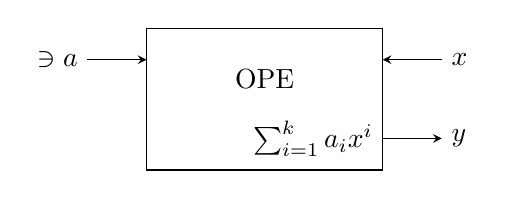
\begin{tikzpicture}[>=stealth]

    \node (OPE) at (8.5,0) {OPE};
    \draw (OPE) +(-1.5,-1.15) rectangle +(1.5,0.65);

    \draw [<-] (OPE) ++(-1.5,0.25) node [anchor=west] {} -- +(-0.75,0) node
    [anchor=east] {$\JWfieldGeneral \ni a$};

    \draw [<-] (OPE) ++(1.5,0.25) node [anchor=east] {} -- +(0.75,0) node
    [anchor=west] {$x$};

    \draw [->] (OPE) ++(1.5,-0.75) node [anchor=east] {$\sum_{i=1}^k a_ix^i$}
    -- +(0.75,0)
    node [anchor=west] {$y$};

  \end{tikzpicture}

  \caption{Graphical Representation of \JWfuncSymOPE}

\end{figure}

\begin{JWprotocol}%
  {\JWprotoSymOPE}%
  {Protocol: Oblivious Polynomial Evaluation}%
  {fig:proto-ope}

  \JWprotoPhase{Setup:}

  \begin{JWprotoSteps}

  \item \JWpOne{} generates the DRAC and sets up the OAFE functionality (see
    section \ref{sec:OPE}).

  \item \JWpOne{} sends DRAC to \JWpTwo{}.

  \end{JWprotoSteps}


  \JWprotoPhase{Evaluation:}

  \begin{JWprotoSteps}

  \item Upon receiving the DRAC, \JWpTwo{} verifies the received input really it
    a DRAC, else ignore that input. Additionally it verifies that the DRAC
    encodes a function whose degree is less or equal than the parametrized
    degree (see chapter \ref{sec:max-poly-degree}), else ignore the input.

  \item After a successful verification, \JWpTwo{} evaluates the DRAC, one DRAE
    after the other. Each DRAE evaluation leads to a DRAV that \JWpTwo{} stores
    as a variable that is used for further computations. Because the OAFE
    functionality is set up by \JWpOne{}, during the evaluation it is possible
    that the OAFE functionality turns out to behave unexpectedly: It could
    decline needed evaluations and it could return vectors of unexpected shapes.
    In both cases always assume it would have returned all zero vectors of the
    expected shape.

  \item After the Evaluation, \JWpTwo{} adds both components of the last DRAV
    and queries a special final OAFE with that value. The then received new
    value is the result of the computation $y = \sum_{i=1}^k a_ix^i$.

  \end{JWprotoSteps}

\end{JWprotocol}

% vim: set spell spelllang=en_us fileencoding=utf8 :
